%%%%%%%%%%%%%%%%%%%%%%%%%%%%%%%%%%%%%%%%%
% University Assignment Title Page 
% LaTeX Template
% Version 1.0 (27/12/12)
%
% This template has been downloaded from:
% http://www.LaTeXTemplates.com
%
% Original author:
% WikiBooks (http://en.wikibooks.org/wiki/LaTeX/Title_Creation)
%
% License:
% CC BY-NC-SA 3.0 (http://creativecommons.org/licenses/by-nc-sa/3.0/)
% 
% Instructions for using this template:
% This title page is capable of being compiled as is. This is not useful for 
% including it in another document. To do this, you have two options: 
%
% 1) Copy/paste everything between \begin{document} and \end{document} 
% starting at \begin{titlepage} and paste this into another LaTeX file where you 
% want your title page.
% OR
% 2) Remove everything outside the \begin{titlepage} and \end{titlepage} and 
% move this file to the same directory as the LaTeX file you wish to add it to. 
% Then add \documentclass[12pt]{article}
\usepackage[english]{babel}
\usepackage{amsmath}
\usepackage{graphicx}
\usepackage{textcomp}
\usepackage{parskip}
\usepackage[colorinlistoftodos]{todonotes}
\usepackage{csquotes}
\usepackage{float}
\usepackage[backend=biber,style=ieee]{biblatex}
\addbibresource{bibliography.bib}

\begin{document}

\begin{titlepage}

\newcommand{\HRule}{\rule{\linewidth}{0.5mm}}
\center 

\textsc{\LARGE Iowa State University }\\[1.5cm] 
\textsc{\Large Center for Statistics and Applications in Forensic
Evidence
}\\[0.5cm] 

\HRule \\[0.4cm]
{ \huge \bfseries Shoe Print Data Collection: Additional Methods }\\[0.4cm] 
\HRule \\[1.5cm]



\begin{center}
\centering
 
\includegraphics[scale=.4]{csafe-logo}\\[1cm]
\end{center}







\end{titlepage}

\section{Introduction}

 When developing the methodology for the longitudinal shoe study conducted by the Center for Statistics and Applications in Forensic Evidence (CSAFE), collection procedures were designed to obtain the most ideal shoe-sole impression possible. While these images will be useful to the researcher and practitioner communities, they do not provide realistic examples of prints that would be collected from a crime scene/suspected crime scene. For this reason, CSAFE researchers have compiled this manual which contains procedures for further data collection and offers new, or edited, procedures that better represent the practices of current forensic examiners and crime scene teams. If at any time there is a question on any of these procedures, please make a note using a post-it note and e-mail the principal investigator, the project manager, the faculty in charge of the study, or the author of the specific procedure. 

\end{document} to your LaTeX file where you want your
% title page.
%
%%%%%%%%%%%%%%%%%%%%%%%%%%%%%%%%%%%%%%%%%
%\title{Title page with logo}
%----------------------------------------------------------------------------------------
%	PACKAGES AND OTHER DOCUMENT CONFIGURATIONS
%----------------------------------------------------------------------------------------

\documentclass[12pt]{article}
\usepackage[english]{babel}
\usepackage[utf8x]{inputenc}
\usepackage{amsmath}
\usepackage{graphicx}
\usepackage[colorinlistoftodos]{todonotes}

\begin{document}

\begin{titlepage}

\newcommand{\HRule}{\rule{\linewidth}{0.5mm}} % Defines a new command for the horizontal lines, change thickness here

\center % Center everything on the page
 
%----------------------------------------------------------------------------------------
%	HEADING SECTIONS
%----------------------------------------------------------------------------------------

\textsc{\LARGE Iowa State University}\\[1.5cm] % Iowa State University 
\textsc{\Large CSAFE}\\[0.5cm] % CSAFE
\textsc{\large Center for Statistics and Applications in Forensic Evidence }\\[0.5cm] % Center for Statistics and Applications in Forensic Evidence 

%----------------------------------------------------------------------------------------
%	TITLE SECTION
%----------------------------------------------------------------------------------------

\HRule \\[0.4cm]
{ \huge \bfseries Paper Powder Print/Vinyl Print: Procedure }\\[0.4cm] % Title of your document
\HRule \\[1.5cm]
 
%----------------------------------------------------------------------------------------
%	AUTHOR SECTION
%----------------------------------------------------------------------------------------

\begin{minipage}{0.4\textwidth}
\begin{flushleft} \large
\emph{Author:}\\
James \textsc{E. Kruse} % Your name
\end{flushleft}
\end{minipage}
~
\begin{minipage}{0.4\textwidth}
\begin{flushright} \large
\emph{Supervisor:} \\
Dr. Guillermo \textsc{Basulto-Elias} % Supervisor's Name
\end{flushright}
\end{minipage}\\[2cm]

% If you don't want a supervisor, uncomment the two lines below and remove the section above
%\Large \emph{Author:}\\
%John \textsc{Smith}\\[3cm] % Your name
%----------------------------------------------------------------------------------------
%	LOGO SECTION
%----------------------------------------------------------------------------------------

\includegraphics[scale=.5]{Logo}\\[1cm]

\begin{center}
\begin{tabular}{ c   |   c } 
 
\end{tabular}
\end{center}
%----------------------------------------------------------------------------------------
%	DATE SECTION
%----------------------------------------------------------------------------------------

{\large \today}\\[2cm] % Date, change the \today to a set date if you want to be precise



 
%----------------------------------------------------------------------------------------

\vfill % Fill the rest of the page with whitespace

\end{titlepage}


\section{Introduction}
***Turn on the lamination machine and allow it to warm up for at least 10-15 min.*** 

1. On a hard surface, pull up a chair. Near by, have a fume hood containing black finger print powder, a cloth, a finger print brush, and a large plastic container (Figure 1). Have an air compressor with a long hose nearby.  

\begin{figure}[!htp]
\centering
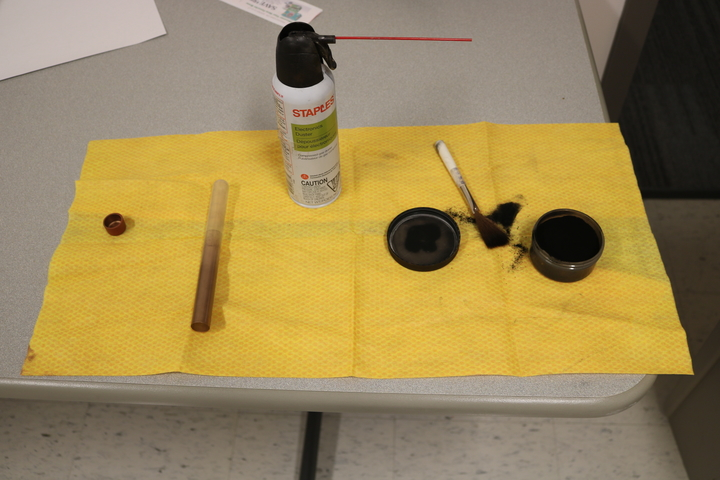
\includegraphics[scale=0.3]{Powder_Stuff}
\caption{Items needed to powder and print.}
\label{Image 1}
\end{figure}

2.	Have the subject sit on the chair, remove a shoe, and loosen the laces.  
3.	Over a trash can, tap the shoe lightly to remove any loose dirt or grass. Some pebbles/dirt that is lodged in the tred is OK and could be a distinguishing characteristic. Under the fume hood and over the plastic container, brush the shoe with print powder. Dip the tip of the brush in the powder and tap the excess off on the side. Carefully, coat the entire shoe out sole in the powder being sure to include all indents, gashes, and grooves (Figure 2).  

\begin{figure}[!htp]
\centering
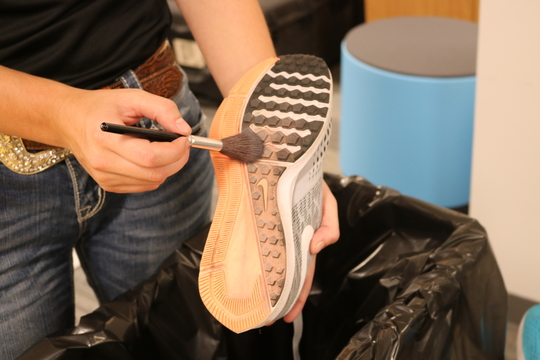
\includegraphics[scale=0.5]{Powder_Brush}
\caption{Completely coat the shoe in powder.}
\label{Image 2}
\end{figure}

\newpage

4. Once the shoe is coated, take the hose of the air compressor and blow off any extra powder. Keep the shoe under the hood while doing this to contain off blowing powder. Be sure to hold the tip a fair distance from the shoe to make sure that all of the powder isn't removed (Figure 3). 

\begin{figure}[!htp]
\centering
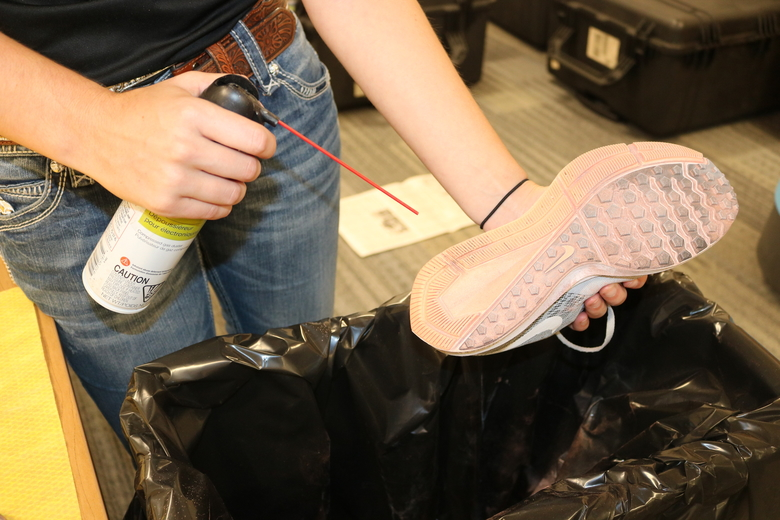
\includegraphics[scale=0.3]{Powder_Air}
\caption{Remove any excess powder.}
\label{Image 3}
\end{figure}

\newpage

5. Return the shoe to the subject and have them put it on. Be sure that nobody touches the sole of the shoe or brushes off any of the powder.

6. At this point, the tech. should put on a pair of disposable gloves. On the ground, place 4 pieces of long printer paper lengthwise, one in front of the other. After the paper, place a piece of the vinyl flooring on the floor (Figure 4). 

\begin{figure}[!htp]
\centering
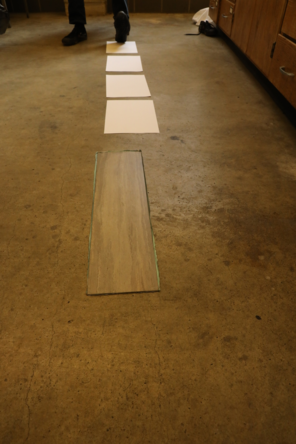
\includegraphics[scale=0.5]{Path}
\caption{Path set up.}
\label{Image 4}
\end{figure}

7. Guide the subjects shoe down onto the paper. The subject should place their heel on the corner of the paper with their toe pointing towards the ceiling. They will then roll their foot into a flat standing position and step up so that all of their weight is on the paper. 



8.Have the subject shift their weight in the shoe in order to capture all detail possible. 

9. Carefully, have the subject step off of the paper. Peel the foot forward until only the tip of the toe is making contact with the paper. At this point, step straight off, but do not place the powdered shoe on the ground (Figure 5). 

\begin{figure}[!htp]
\centering
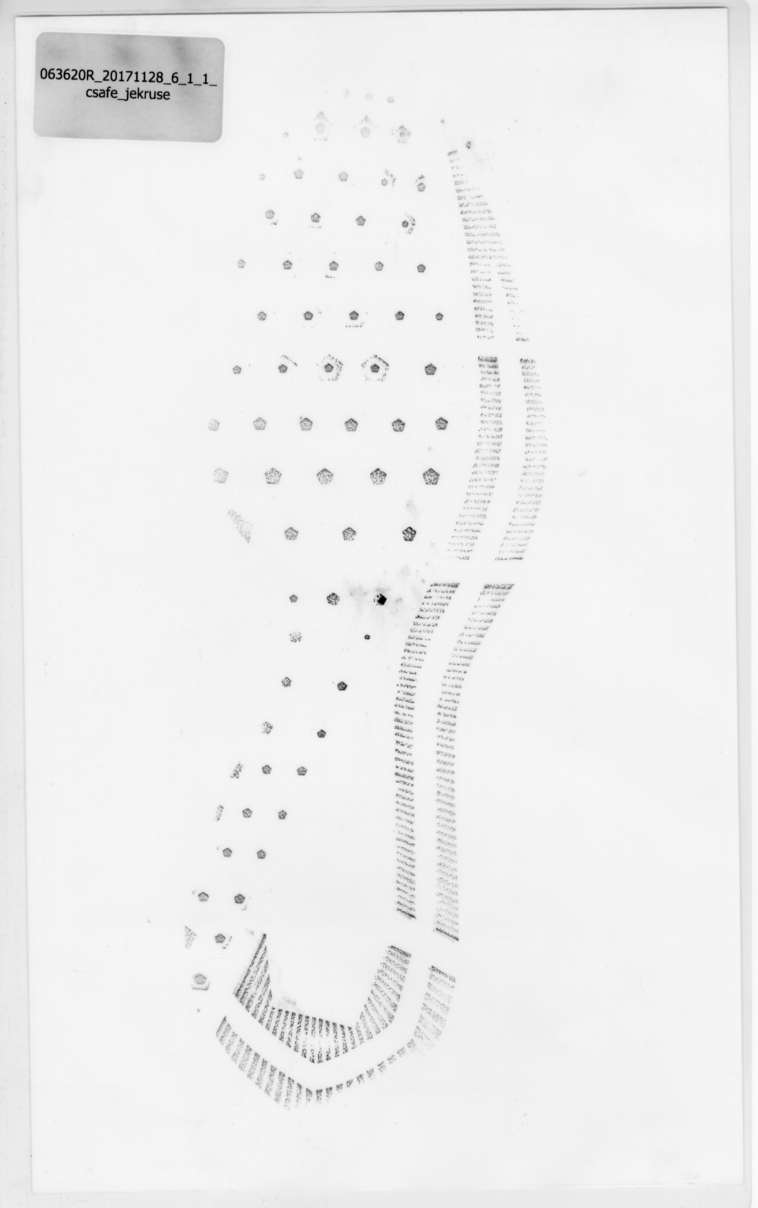
\includegraphics[scale=0.2]{Baseline_Paper_1}
\caption{Completed image 1}
\label{Image 5}
\end{figure}

\newpage

10. On the second paper, Position the foot in the same way, but take a step as if walking normally. Again, do not place the powdered shoe on the ground after the print has been taken (Figure 6). 


\begin{figure}[!htp]
\centering
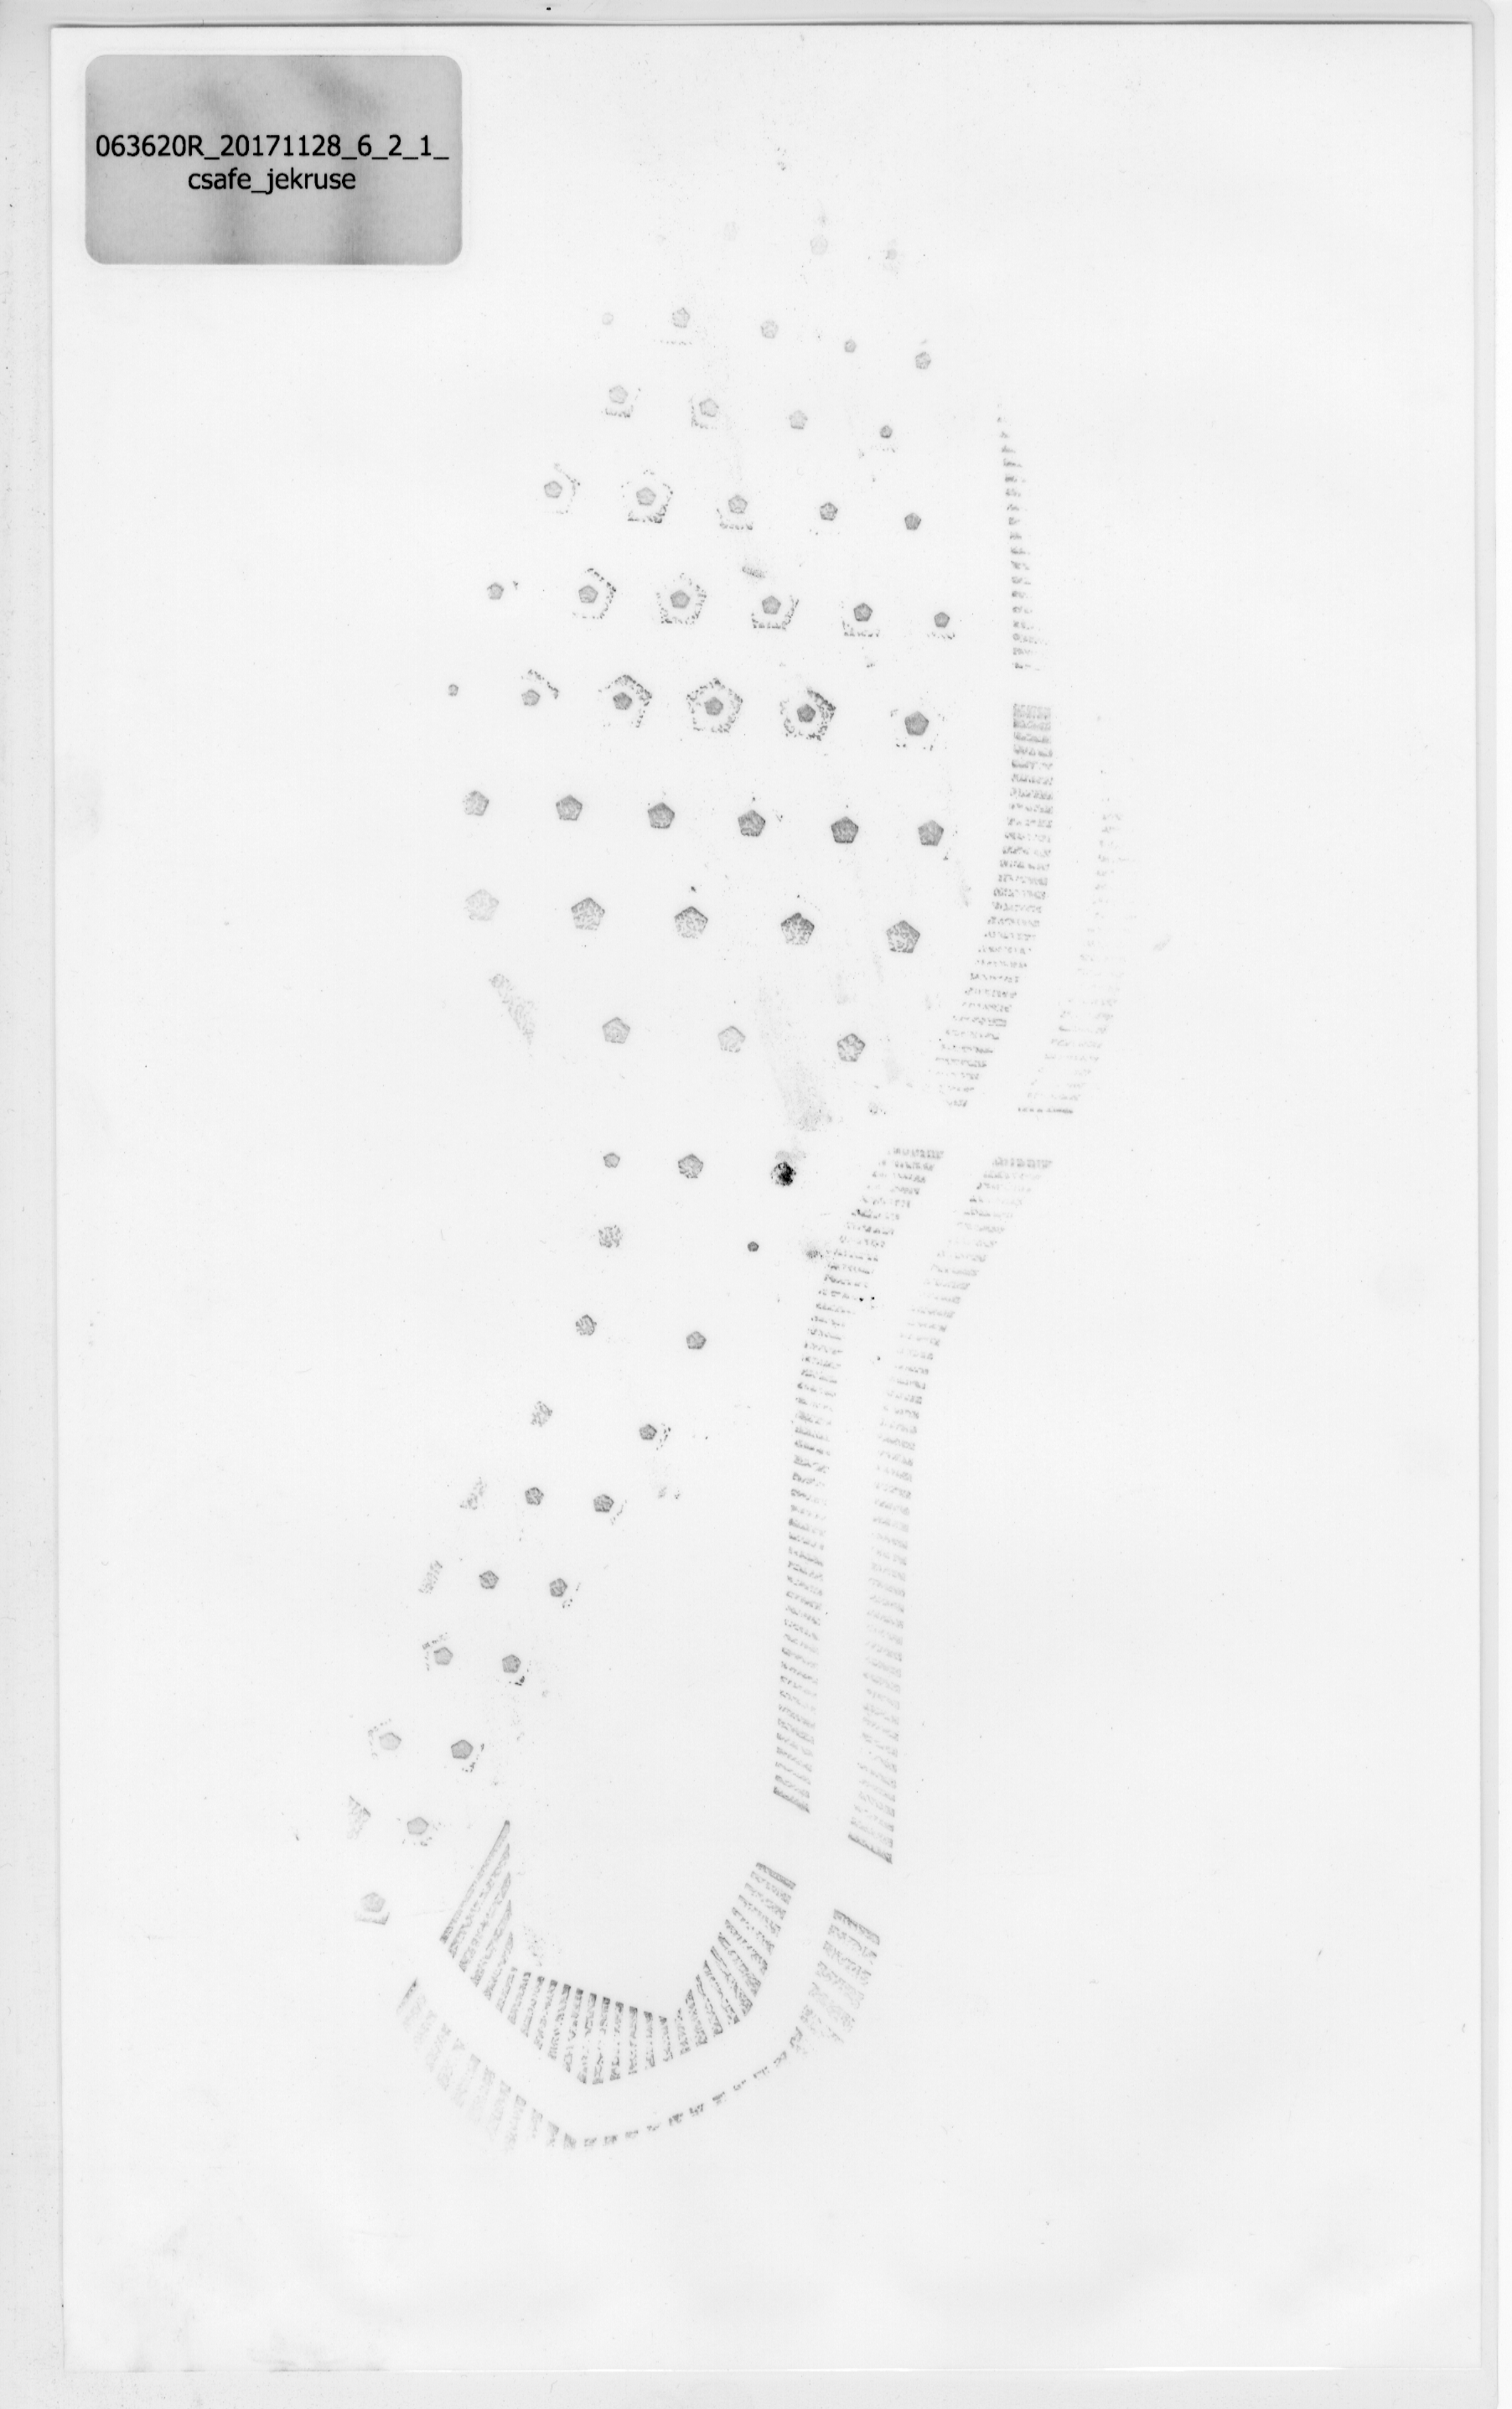
\includegraphics[scale=0.1]{Baseline_Paper_2}
\caption{Completed image 2}
\label{Image 6}
\end{figure}

12. On the third paper, have the subject stamp their foot straight down. Make sure that the foot is completely captured on the paper and that no part is missing. Lift the shoe straight into the air (Figure 7), but do not place the powdered shoe on the ground (Figure 8).

\begin{figure}[!htp]
\centering
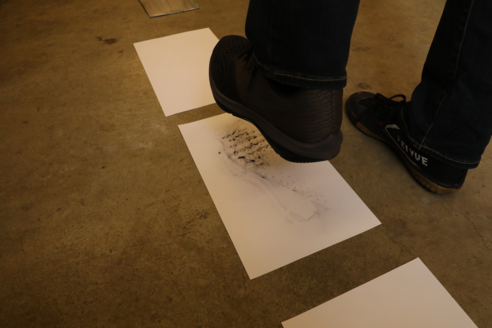
\includegraphics[scale=0.4]{Stomp}
\caption{Taking the third print}
\label{Image 7}
\end{figure}

\begin{figure}[!htp]
\centering
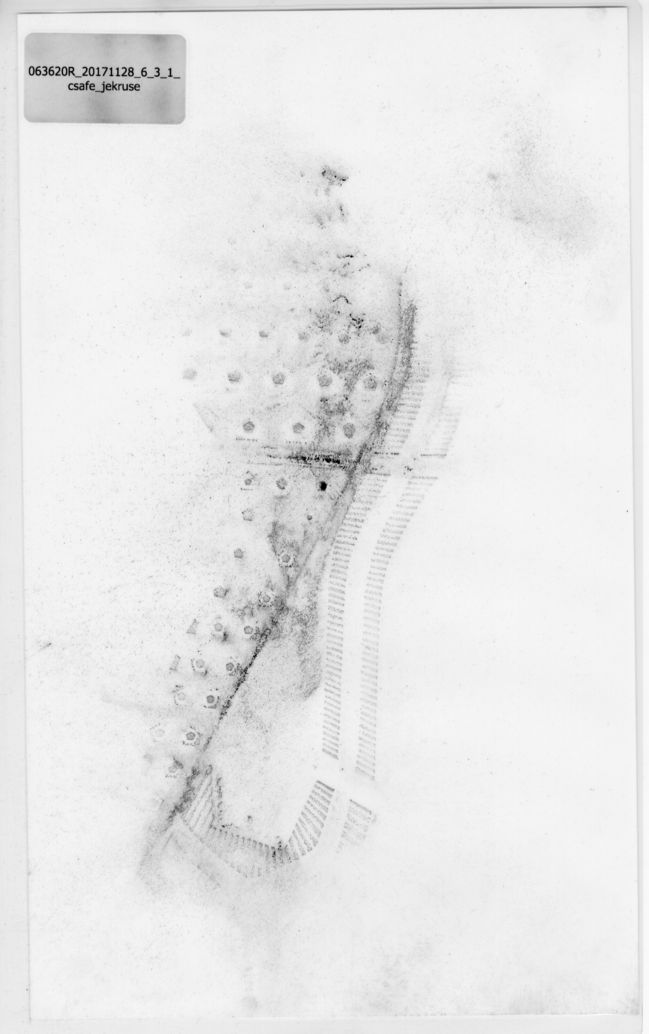
\includegraphics[scale=0.3]{Baseline_Paper_3}
\caption{Completed image 3}
\label{Image 8}
\end{figure}

13. On the fourth paper, have the subject step and slightly twist, to smudge the print. Then step straight off, but do not place the powdered shoe on the ground (Figure 9)

\begin{figure}[!htp]
\centering
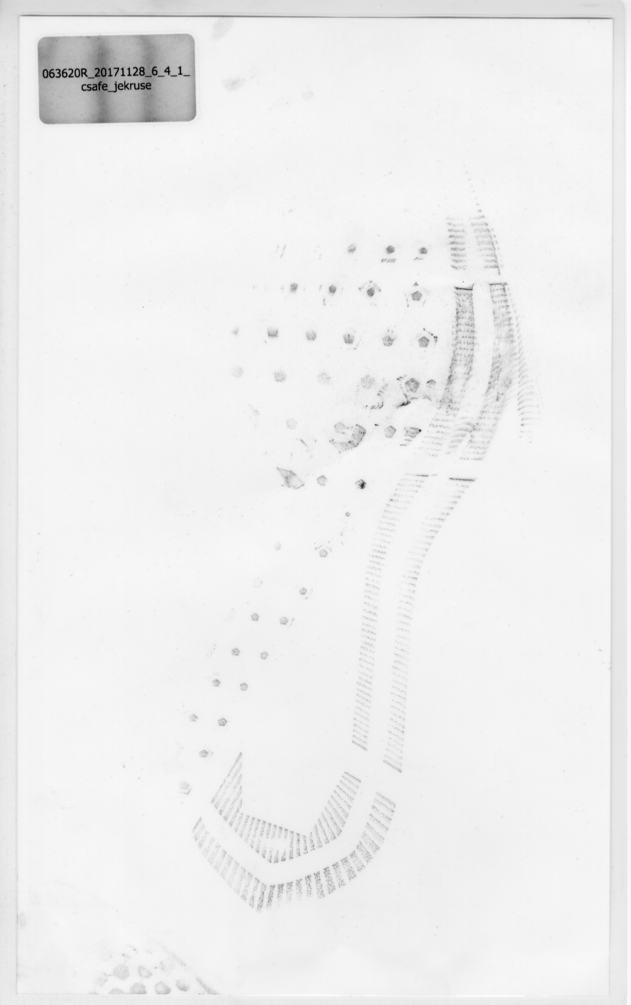
\includegraphics[scale=0.3]{Baseline_Paper_4}
\caption{Completed image 4}
\label{Image 9}
\end{figure}

\newpage

14. Lastly, have the subject walk across the vinyl flooring in the same way that they did for the second sheet of paper. 

15. Please see the naming key on the back of the manual cover for full naming criteria. Use the naming tool created by IT to generate the name. Copy and paste that name into the label maker. Behind the subjects name, ad an underscore and put the techs name. If this is the same person, put the name twice. Then press print, and place the label in an upper corner not occupied by the print.With a dry erase marker, label the bottom of the vinyl flooring using the vinyl flooring name from the key.


16. Carefully open the laminate pouch and place the print in with the sticker/tip of the shoe toward the crease, making sure to not smudge or damage the print. Place the print in the laminate machine crease down and allow it to feed through, making sure that it stays straight. 



17. Place the scans in the correct files for later scanning. Place the vinyl flooring aside for later photos. 

Note: For paper print scanning Please refer to the bed scanner procedure. For flooring photos, refer to the Vinyl photo Procedure. 

\end{document}